%Version 2.1 April 2023
% See section 11 of the User Manual for version history
%
%%%%%%%%%%%%%%%%%%%%%%%%%%%%%%%%%%%%%%%%%%%%%%%%%%%%%%%%%%%%%%%%%%%%%%
%%                                                                 %%
%% Please do not use \input{...} to include other tex files.       %%
%% Submit your LaTeX manuscript as one .tex document.              %%
%%                                                                 %%
%% All additional figures and files should be attached             %%
%% separately and not embedded in the \TeX\ document itself.       %%
%%                                                                 %%
%%%%%%%%%%%%%%%%%%%%%%%%%%%%%%%%%%%%%%%%%%%%%%%%%%%%%%%%%%%%%%%%%%%%%

%%\documentclass[referee,sn-basic]{sn-jnl}% referee option is meant for double line spacing

%%=======================================================%%
%% to print line numbers in the margin use lineno option %%
%%=======================================================%%

%%\documentclass[lineno,sn-basic]{sn-jnl}% Basic Springer Nature Reference Style/Chemistry Reference Style

%%======================================================%%
%% to compile with pdflatex/xelatex use pdflatex option %%
%%======================================================%%

%%\documentclass[pdflatex,sn-basic]{sn-jnl}% Basic Springer Nature Reference Style/Chemistry Reference Style


%%Note: the following reference styles support Namedate and Numbered referencing. By default the style follows the most common style. To switch between the options you can add or remove “Numbered” in the optional parenthesis. 
%%The option is available for: sn-basic.bst, sn-vancouver.bst, sn-chicago.bst, sn-mathphys.bst. %  
 
%%\documentclass[sn-nature]{sn-jnl}% Style for submissions to Nature Portfolio journals
%%\documentclass[sn-basic]{sn-jnl}% Basic Springer Nature Reference Style/Chemistry Reference Style
% \documentclass[sn-mathphys,Numbered]{sn-jnl}% Math and Physical Sciences Reference Style
%%\documentclass[sn-aps]{sn-jnl}% American Physical Society (APS) Reference Style
%%\documentclass[sn-vancouver,Numbered]{sn-jnl}% Vancouver Reference Style
%%\documentclass[sn-apa]{sn-jnl}% APA Reference Style 
%%\documentclass[sn-chicago]{sn-jnl}% Chicago-based Humanities Reference Style
%%\documentclass[default]{sn-jnl}% Default
\documentclass[default,iicol]{sn-jnl}% Default with double column layout

%%%% Standard Packages
%%<additional latex packages if required can be included here>

\usepackage{graphicx}%
\usepackage{multirow}%
\usepackage{amsmath,amssymb,amsfonts}%
\usepackage{amsthm}%
\usepackage{mathrsfs}%
\usepackage[title]{appendix}%
\usepackage{xcolor}%
\usepackage{textcomp}%
\usepackage{manyfoot}%
% \usepackage{booktabs}%
\usepackage{algorithm}%
\usepackage{algorithmicx}%
\usepackage{algpseudocode}%
\usepackage{listings}%
\usepackage{array}  
\usepackage{listings}
% \usepackage{tabulary}

\catcode`\|=12\relax % added  <<<<<<<<<<<<<<<<<
\usepackage{orcidlink} % added <<<<<<<<<<<<


\lstset{ %
	language=Python,                     % choose the language of the code
	basicstyle=\footnotesize,       % the size of the fonts that are used for the code
	numbers=left,                   % where to put the line-numbers
	numberstyle=\footnotesize,      % the size of the fonts that are used for the line-numbers
	stepnumber=2,                   % the step between two line-numbers. If it's 1 each line will be numbered
	numbersep=5pt,                  % how far the line-numbers are from the code
	backgroundcolor=\color{white},  % choose the background color. You must add \usepackage{color}
	showspaces=false,               % show spaces adding particular underscores
	showstringspaces=false,         % underline spaces within strings
	showtabs=false,                 % show tabs within strings adding particular underscores
	frame=single,                  % adds a frame around the code
	tabsize=2,                    % sets default tabsize to 2 spaces
	captionpos=b,                   % sets the caption-position to bottom
	breaklines=true,                % sets automatic line breaking
	breakatwhitespace=false,        % sets if automatic breaks should only happen at whitespace
	escapeinside={\%*}{*)}          % if you want to add a comment within your code
}

%%%%
\renewcommand{\L}{\mathcal{L}}
\renewcommand{\a}{\alpha}
\renewcommand{\b}{\beta}
\newcommand{\R}{\mathcal{R}}
\def\Dot#1{\overset{\hbox{\tiny$\bullet$}}{#1}}

\DeclareRobustCommand{\bbone}{\text{\usefont{U}{bbold}{m}{n}1}}

\DeclareMathOperator{\EX}{\mathbb{E}}
\DeclareMathOperator{\VAR}{\mathbb{V}}

%%%%%=============================================================================%%%%
%%%%  Remarks: This template is provided to aid authors with the preparation
%%%%  of original research articles intended for submission to journals published 
%%%%  by Springer Nature. The guidance has been prepared in partnership with 
%%%%  production teams to conform to Springer Nature technical requirements. 
%%%%  Editorial and presentation requirements differ among journal portfolios and 
%%%%  research disciplines. You may find sections in this template are irrelevant 
%%%%  to your work and are empowered to omit any such section if allowed by the 
%%%%  journal you intend to submit to. The submission guidelines and policies 
%%%%  of the journal take precedence. A detailed User Manual is available in the 
%%%%  template package for technical guidance.
%%%%%=============================================================================%%%%

%\jyear{2021}%

%% as per the requirement new theorem styles can be included as shown below
\usepackage{xparse}

\newcolumntype{L}[1]{>{\raggedright\let\newline\\\arraybackslash\hspace{0pt}}m{#1}}
\newcolumntype{C}[1]{>{\centering\let\newline\\\arraybackslash\hspace{0pt}}m{#1}}
\newcolumntype{R}[1]{>{\raggedleft\let\newline\\\arraybackslash\hspace{0pt}}m{#1}}

\NewDocumentCommand{\codeword}{v}{%
\texttt{{#1}}%
}
% \usepackage{listings}
\lstMakeShortInline[language=Matlab]|
\newcommand\inlineMatlab[2][]{\lstinline[language=Matlab,#1]+#2+}


\newcommand\MyBox[2]{
  \fbox{\lower0.75cm
    \vbox to 1.2cm{\vfil
      \hbox to 1.2cm{\hfil\parbox{1.2cm}{\centering #1\\#2}\hfil}
      \vfil}%
  }%
}

% \makeatletter
% \newcommand{\customlabel}[2]{%
% \protected@write \@auxout {}{\string \newlabel {#1}{{#2}{}}}}
% \makeatother

% \newcounter{NameOfTheNewCounter}
% \renewcommand{\theNameOfTheNewCounter}{MIS-{\ifnum\value{NameOfTheNewCounter}<100 0\fi}\arabic{misreqs}}
% \newcommand{\NameOfTheNewCounterCnt}[1]{%
%   \addtocounter{NameOfTheNewCounter}{10}% Step counter
%   \theNameOfTheNewCounter% Print counter
%   \addtocounter{NameOfTheNewCounter}{-1}\refstepcounter{NameOfTheNewCounter}\label{#1}}% Mark with label

% \newcommand{\missionrequiremententries}{}
% \newcommand{\customlabel}[1]{%
% \protected@xdef\missionrequiremententries{\missionrequiremententries \protect\misreqCnt{#1} \protect\\}}


\newenvironment{confusionMat}[9]
{
% \captionsetup{width=\textwidth}
\begin{table}[ht]
% \noindent
\centering
\renewcommand\arraystretch{1.5}
\setlength\tabcolsep{0pt}
\resizebox{.2\textwidth}{!}{
\begin{tabular}{c @{\hspace{1.1em}}>{\bfseries}r @{\hspace{.7em}}c @{\hspace{0.4em}}c}
  \multirow{9}{*}{\rotatebox{90}{\parbox{5cm}{\bfseries\centering Predicted Class}}} & 
    & \multicolumn{2}{c}{\bfseries True Class} \\
  & & \bfseries 0 & \bfseries 1 \\
  & 0 & \MyBox{#1}{(#2\%)} & \MyBox{#3}{(#4\%)} \\[3em]
  & 1 & \MyBox{#5}{(#6\%)} & \MyBox{#7}{(#8\%)}  \\[4.5em]
\end{tabular}}
\caption{#9}
% \customlabel{#10}
% \customlabel{#10}{#11}
% \customlabel{#10}
\end{table}
}
{
}


% \theoremstyle{thmstyleone}%
\newtheorem{theorem}{Theorem}%  meant for continuous numbers
%%\newtheorem{theorem}{Theorem}[section]% meant for sectionwise numbers
%% optional argument [theorem] produces theorem numbering sequence instead of independent numbers for Proposition
\newtheorem{proposition}[theorem]{Proposition}% 
%%\newtheorem{proposition}{Proposition}% to get separate numbers for theorem and proposition etc.

% \theoremstyle{thmstyletwo}%
\newtheorem{example}{Example}%
\newtheorem{remark}{Remark}%

% \theoremstyle{thmstylethree}%
\newtheorem{definition}{Definition}%

\raggedbottom
%%\unnumbered% uncomment this for unnumbered level heads
\linespread{1.5}
\begin{document}

\title[Application of LSTM Neural Network in Optimizing-then-Predicting Winning and Losing Stocks]{Application of LSTM Neural Network in Optimizing-then-Predicting Winning and Losing Stocks}

%%=============================================================%%
%% Prefix	-> \pfx{Dr}
%% GivenName	-> \fnm{Joergen W.}
%% Particle	-> \spfx{van der} -> surname prefix
%% FamilyName	-> \sur{Ploeg}
%% Suffix	-> \sfx{IV}
%% NatureName	-> \tanm{Poet Laureate} -> Title after name
%% Degrees	-> \dgr{MSc, PhD}
%% \author*[1,2]{\pfx{Dr} \fnm{Joergen W.} \spfx{van der} \sur{Ploeg} \sfx{IV} \tanm{Poet Laureate} 
%%                 \dgr{MSc, PhD}}\email{iauthor@gmail.com}
%%=============================================================%%

\author{\fnm{Duan} \sur{Linjia}}

\affil{\orgdiv{National University of Singapore (Suzhou) Research Institute}}



%%==================================%%
%% sample for unstructured abstract %%
%%==================================%%

\abstract{In the stock market, investors usually choose to bet on several stocks at the same time instead of just invest the stock with highest returns to increase the risk tolerance. According to modern portfolio theory, they tend to select a particular portfolio according to their aversion to risk from the efficient frontier in Markowitz's mean-variance model. In the efficient frontiers derived from the model, each expected return correspond its lowest volatility, which means the portfolio is ‘optimal’. However, we can find some stocks that are included in most portfolios on efficient frontier and some stocks that are excluded in the vast majority of portfolios. We call them "winners" and "losers" based on whether we invest them in a portfolio. Determining winners and losers in the stock market will help us to trade more efficiently and increase the likelihood of making a profit. We aim to utilize the relevant data in stock market to obtain the efficient frontiers and clear whether the specific stock is included or excluded in optimal portfolio to make a supervised machine learning for a well-designed neural network model to predict the potential winners and losers in the stock market and whether a new stock entering the market is winner or loser. Investors could use the model to invest more efficiently and get higher returns in a specific risk level.}


\keywords{Optimal portfolio, Markowitz's mean-variance model, Machine learning, Neural network}

%%\pacs[JEL Classification]{D8, H51}

%%\pacs[MSC Classification]{35A01, 65L10, 65L12, 65L20, 65L70}

\maketitle
\clearpage
\onecolumn
\tableofcontents  % 生成目录
\clearpage
\twocolumn
\bmhead{Acknowledgments}

Throughout the writing of this dissertation I have received a great deal of support and assistance from my supervisor, Napat RUJEERAPAIBOON. I would like to thank him for his expertise that helps a lot in formulating the research program and the method. His feedback inspired me a lot when I was challenged with the project and allowed me to continue my research.

\section{Introduction}\label{sec1}


\hspace{1.5em}The Markowitz mean-variance portfolio optimization model \cite{1952Portfolio} is designed to weigh the expected return and risk when investing. Investors with different levels of risk aversion have the option of choosing different portfolios according to their objectives, thus constructing an optimal portfolio with efficient frontiers that represent all possible risk tolerances \cite{2009Investment}.

Based on this fact, we research the domestic A-share market using a miniature simulated stock market consisting of fifty randomly selected stocks from the Shanghai and Shenzhen markets. Based on the mean-variance model, we can obtain all the decisions that a rational investor can make, that is the efficient frontier, and the weight share of each stock in these portfolios. It could help us establish a threshold to determine whether stocks are overwhelmingly included or excluded, the winners or losers, based on these weightings.

Most of the current research is on optimal robust portfolios in stock markets in different regions to realize the selection of stocks in specific circumstances \cite{2019Application,lee2024comparison}. Furthermore, machine learning in the field of stocks, especially artificial neural networks, are more often used for time series forecasting of stock prices \cite{2016Application,2022Robust}.

We construct a neural network with long short-term memory algorithms based on previous research on neural network models and machine learning optimization \cite{2005A,2010Rectified,2014Adam,1997Long}. We build a simulated miniature market for machine learning, where we consider a brand new stock as a new stock flowing into this market for forecasting. It is possible to make a prediction about one stock by inputting the average daily return \cite{1988Game} of a stock over a past time period to determine whether it has a greater likelihood of being a loser or a winner.

\section{Literature Review}\label{sec2}

\hspace{1.5em}For this project, I have selected fifty stocks to form a simulated miniature stock market. I first needed to analyze how an investor would select stocks to invest in this stock market. Markowitz published \textit{"Portfolio selection"} in 1952 \cite{1952Portfolio}, which quantifies an investor's choice as a trade-off between risk and return, a quadratic programming problem. According to the modern portfolio theory, a rational investor will choose the portfolio with the highest benefit according to different risk aversion, that is the mean-variance model. Luenberger wrote a book, \textit{"Investment Science"}, in the 1997, the chapter 6 of the book explains in detail the use of mean-variance portfolio theory in the actual market and the underlying logic \cite{2009Investment}. Using the Markowitz model, I was able to obtain the optimal investment weights for each stock in the simulated market under different levels of risk for this project. Zhang Chern Lee utilized the portfolio theory to analyze the Malaysian stock market with the aim of constructing an effective portfolio using the Markowitz model as well as Sharpe's mono-exponential model in order to provide effective information to the investors concerned \cite{lee2024comparison}. It inspires me to analyze the simulated stock market to some extent. At the same time, Chao’s research \cite{2019Application} shows that mean-variance model can be well applied to the domestic A-share market and can be used to obtain various portfolios selected by different investors in the market. The overall profitability of Markowitz capital portfolio in the domestic A-share market exceeds the portfolio currently used by the securities market.

It turns out however that some particular stocks may be included in most times, which could be seen as winners, whereas some others should hardly never be considered, which is losers. In practice, it turns out that many stocks are losers while a little stocks are winners. Finding them could improve the efficiency of algorithmic trading. Machine learning is a good method for predicting potential losers and winners in a portfolio. Cassidy K. Buhler constructed a predictive model of whether stocks are included in a portfolio in June 2023, and he also sparsified the large and dense covariance matrix in the large portfolio problem to optimize the model \cite{buhler2023efficient}. His research is similar to the losing stocks defined in this program, however, he did not make effective predictions for stocks that are most times included in portfolios. Fu XingYu, in his August 2018 article, \textit{"A Machine Learning Framework for Stock Selection"} \cite{fu2018machine}, performed a deep feature based on genetic algorithm engineering and utilized the resulting 244 features for various algorithms such as Logistic Regression, Random Forest, Neural Network, to predict the "good" and "bad" stock according to their ranking with respect to the return-to-volatility ratio. His research inspired the choice of algorithms to recognize the winners and losers.

Regarding the specific construction of machine learning models, it is mainly categorized into data processing as well as model construction. The closing price of a stock needs to be processed as the expected return for the construction of the efficient frontier. Neural networks are very popular learning algorithms in recent years. Qiu Mingyue's research utilized artificial neural networks to predict the direction of stock market indices, while Jaydip Sen also utilized neural networks to implement robust portfolio design and stock price prediction \cite{2016Application,2022Robust}. Their research directions are related with my program and neural network models are more popular in stock market prediction, so my program mainly focuses on the construction of artificial neural networks. S. Hochreiter proposed the far-reaching Long and Short-Term Memory (\textit{LSTM}) model in 1997, which endows neural networks with the function of remembering and forgetting, allowing the model to have a key feature of "deeper memory" \cite{1997Long}. The daily return in this project is a time-series based feature, and the Long Short-Term Memory model is even more powerful for this type of data. Jaydip Sen's research about portfolio design and Cassidy K. Buhler's research about portfolio excluded stocks prediction are based on building neural networks based on the LSTM model \cite{2022Robust,buhler2023efficient}. In addition, D.A. Tadesse and others, in a paper published in 2020, argued that the results of time series analysis of financial historical data based on basic statistical techniques are limited. LSTM has a strong advantage in the predictive construction and optimization of efficient portfolio \cite{2020Portfolio}. His view and the study of T. Fischer in 2018 both proved that LSTM has a better predictive effect on financial data \cite{2018Deep}. Gradient descent in neural networks is a very important optimization method used to search for suitable parameters to minimize the cost function. D Kingma in his 2014 article \textit{“Adam: A Method for Stochastic Optimization”} proposed Adam's algorithm, which is a much more powerful optimization algorithm that automatically adjusts the learning rate when the learning rate is too big or too small \cite{2014Adam}. In addition, the activation function in the input layer, output layer and hidden layer of the neural network is also an important indicator. V. Nair published a paper in 2010 proposing a rectified linear function (\textit{ReLU}), which can perform gradient descent and backpropagation more efficiently than the traditional linear function, avoiding the problem of gradient explosion and gradient disappearance \cite{2010Rectified}. The following papers also inspired me a lot about the selection of some parameters, such as batch size, the usage of regularization and the cross entropy function when constructing neural network \cite{smith2018dont,2009L2,2005A}.

Moreover, in A. Geron's book in 2017, \textit{"Hands-On Machine Learning with Scikit-Learn, Keras, and Tensorflow"} provides an detailed introduction to the various machine learning frameworks in python and their implementation processes \cite{Aur2017Hands}.

\section{Mean-variance Model}\label{sec3}

In this section, we present the mean-variance model we used in detail.

\subsection{Assumptions}\label{sec3sub1}
\begin{enumerate}
    \item Investors consider each investment choice based on the probability distribution of returns within a specific time period.
    \item All investors are "rational" which means they focus only on the  risk and expected return. At a given level of risk, investors expect maximum return; correspondingly, at a given level of returns, investors expect minimum risk.
    \item There are no extra fees, such as taxes, in the trading process, and there are no restrictions on entering or leaving the market.
    \item Investors use the volatility of the expected rate of return to assess the risk of the portfolio \cite{2019Application}.
\end{enumerate}

\subsection{Model Construction}\label{sec3sub2} 
In the construction part of the model, we convert most of the formulas into a matrix form to express, for example, the weights of the stocks in the portfolio. Because matrix multiplication in a computer can effectively utilize the performance of the GPU to achieve large-scale operations, which helps to improve the efficiency of the entire program.
\subsubsection{Returns}\label{sec3sub2ssub1}
\hspace{1.5em}We first use raw data that can be obtained from the internet, the daily closing price of a stock, as an indicator to calculate the return of each stock in the simulated stock market. We chose to use the rate of return function to measure the stock's return:
\begin{align}
	r_{i,t}=\frac{p_{i,t}-p_{i,t-1}}{p_{i,t-1}}
	\label{eq1}
\end{align}

Using the obtained stock returns, we can calculate the average return of each stock in a long time series, as well as the expected overall return of the entire portfolio: 
\begin{align}
	\mu _{i}=\sum_{t-2}^{T}r_{i,t}, \hspace{1em}\mathbb{E}(R)=\sum_{i=1}^{50}\mu_{i}w _{i}=\mu ^{T}w  
	\label{eq2}
\end{align}
\subsubsection{Variance}\label{sec3sub2ssub2}
\hspace{1.5em}We need to define the formula for covariance, which is used to calculate the large covariance matrix in the portfolio:
\begin{align}
	\sigma _{ij} =E(r_{i,t}\times r_{j,t})-\mu_{i}\mu_{j}
	\label{eq3}
\end{align}

Based on the covariance formula, we can calculate the variance of the entire portfolio and represent it as a matrix:
\begin{align}
	\mathbb{V}(R)=\sum_{i,t=1}^{n} w_{i} w _{j}\sigma _{ij} =w ^{T}cov(R)w  
	\label{eq4}
\end{align}

\subsubsection{Mean-variance Model and Efficient frontiers}\label{sec3sub2ssub3}
\hspace{1.5em}Using the above calculations, we could implement the Markowitz model \cite{1952Portfolio}:

\begin{equation}
\begin{aligned}
	\min_{w } \quad &\sqrt{w^{T} cov(R)w } \\
	\textrm{s.t.}  \quad & \mu^{T}w = \bar{R} \\
	& \sum_{i=1}^{n}w_{i}=1 
	\label{eq5}
\end{aligned}
\end{equation}

When we set a proper array of fixed target expected value in the Markowitz model, we can obtain all optimal portfolios and represent them as efficient frontiers.

In the Markowitz model, expected returns are measured in this program as the average of historical returns, while risk is interpreted as volatility \cite{2009Investment}. The covariance matrix we use can be used to obtain the variance of individual portfolio returns across the efficient frontier.

The efficient frontier is composed of Volatility ($w^{T} cov(R)w$) and Risk ($\mu^{T}w$), which respectively represent the profitability and volatility probability of an specific portfolio. All optimal portfolio points should be on the boundary formed by a convex curve, whereas all points inside the boundary are considered to be "inefficient". Which point on the efficient frontier is used depends on the investor's preference.

\section{Data and Methodology}\label{sec4}
\subsection{Data Collection}\label{sec4sub1}
\hspace{1.5em}In this program, 50 stocks are randomly selected from the Shanghai and Shenzhen stock markets to form a miniature simulation market as the research object, such as 000001 (Ping An Bank), 600000 (Pudong Development Bank) and other representative stocks. The detailed daily, weekly and monthly quotes of these stocks between 9 January 2020 and 28 February 2024 are obtained from the stock trading database of the Tushare website. During this period, there were 801 trading days. Stock profitability is expressed in terms of annual, monthly, weekly and daily rates. Investors usually use the daily quotes to make specific point selections after confirming the direction of the weekly and monthly quotes. Since the focus of the program is on the investor's choices in the portfolio, we choose the daily rate to analyze. From Tushare database, we apply to call the daily closing price of the target stock in the period. The result shows in Figure \ref{fg1}.

\begin{figure*}[h]
	\centering    
	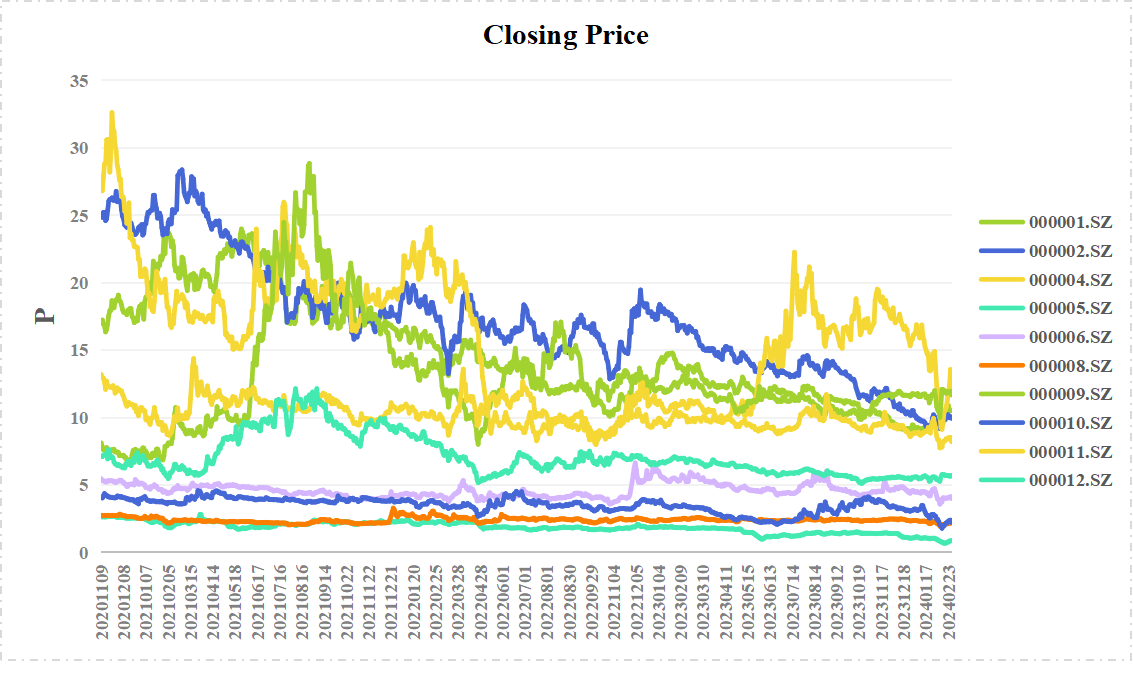
\includegraphics[width = 0.6\textwidth]{figures/Fig 1.png}
	\caption{The daily closing prices of ten stocks are shown to reflect the trend of stock prices. There are too many target stocks therefore only some of them are selected for visualization.}
	\label{fg1}
\end{figure*}  

\subsection{Data Processing}\label{sec4sub2}
\hspace{1.5em}Calculate the daily returns of 50 stocks over the sample time period according to Equation \eqref{eq5}. We obtain a matrix of the returns of different stocks under different dates as Table \eqref{tab1}.
\begin{table}[htbp]
	\centering  
	\begin{tabular}{|c|c|c|c|c|}  
		\hline  % 表格的横线
		& & & &\\[-6pt]  %可以避免文字偏上来调整文字与上边界的距离
		\textbf{trade date}&\textbf{20201110}&\textbf{20201111}&...&\textbf{20240228} \\  
		\hline
		& & & & \\[-6pt]
		\textbf{000001.SZ}&0.0093107&-0.0013229&...&0.0009528 \\
		\hline
			& & & & \\[-6pt]
		\textbf{000002.SZ}&-0.0139716&0.0037819&...&-0.0130067 \\
		\hline
		& & & & \\[-6pt]
		...&...&...&...&... \\
		\hline
		& & & & \\[-6pt]
		\textbf{600088.SH}&0.017354&0.0053619&...&-0.10522788 \\
		\hline
	\end{tabular}
\caption{Matrix of the stock returns by date (Partial)} 
\label{tab1}
\end{table}

Calculate the standard deviation of the returns over the sample time period:
\begin{align}
	\sigma _{i} & = \sqrt{\frac{\sum_{1}^{I} (\mu_{i}-r_{i,t})^2}{I} } 
	\label{eq6}
\end{align}

Calculate the covariance of the returns of the sample stocks according to Equation \eqref{eq3}. Again, we get a large and dense covariance matrix. The sample covariance matrix are finally computed as shown in Table \eqref{tab2}.
\begin{table}[htbp]
	\centering  
	\begin{tabular}{|c|c|c|c|c|}  
		\hline  % 表格的横线
		& & & &\\[-6pt]  %可以避免文字偏上来调整文字与上边界的距离
		 &\textbf{000001.SZ}&\textbf{000002.SZ}&...&\textbf{600088.SH} \\  
		\hline
		& & & & \\[-6pt]
		\textbf{000001.SZ}&0.000406&0.00024284&...&7.25494e-05 \\
		\hline
		& & & & \\[-6pt]
		\textbf{000002.SZ}&0.00024284&0.00049246&...&6.6805e-05 \\
		\hline
		& & & & \\[-6pt]
		...&...&...&...&... \\
		\hline
		& & & & \\[-6pt]
		\textbf{600088.SH}&7.25494e-05&6.6805e-05&...&0.0010024 \\
		\hline
	\end{tabular}
	\caption{Matrix of covariance between sample stocks (Partial)} 
	\label{tab2}
\end{table}

Take the above data into the Markowitz model, and use Python tools to model it through Algorithm \ref{al1}. We obtain the efficient frontiers as Figure \ref{fg2} and weights that all sample stocks occupy in the different portfolios of the efficient frontier.
\begin{algorithm}
	\caption{Effective frontier modeling under mean-variance models}
	\label{al1}
	\begin{algorithmic}[1]
		\State Call the data using the library corresponding to Tushare.
		\State Process the data according to Equations \eqref{eq1} \eqref{eq2} \eqref{eq3} \eqref{eq6}
		\State Define the portfolio annualized return $\mathbb{E}(R)$ and standard deviation $\mathbb{V}(R)$
		\State Build the quadratic programming of the mean-variance model by Equation \eqref{eq5}
		\State Derive an array of efficient frontiers with fixed target returns.
		\State Derive specific weights for different portfolios on the efficient frontier
	\end{algorithmic}
\end{algorithm}

\begin{figure*}[h]
	\centering    
	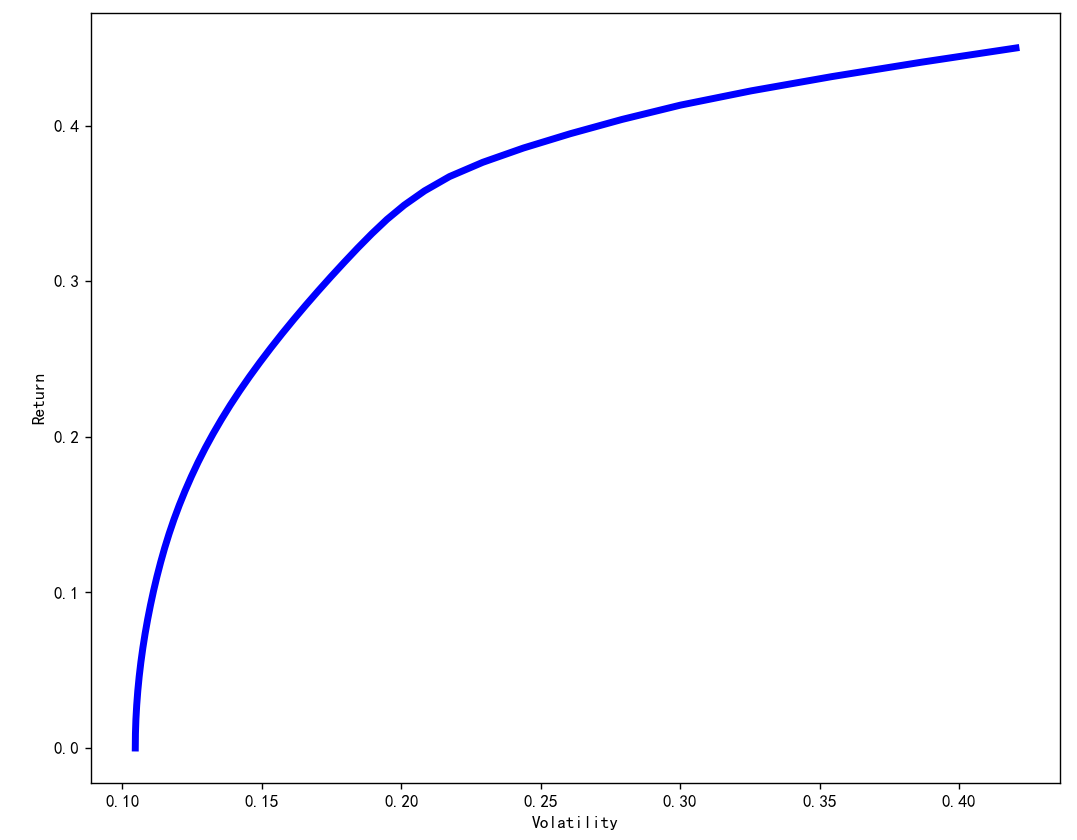
\includegraphics[width = 0.6\textwidth]{figures/Fig 2.png}
	\caption{The efficient frontier of 50 stocks randomly selected from the Shanghai and Shenzhen stock markets using daily returns from 9 January 2020 to 28 February 2024 (Returns and Volatility are processed as annualized by 252 trading day)}
	\label{fg2}
\end{figure*} 

\subsection{Dataset Collation}\label{sec4sub3}
\hspace{1.5em}We make judgements according to the weight that a specific stock holds in the portfolio. Distributing the weights evenly to each stock in a portfolio is the standard case. Therefor we determine whether a stock is included in a portfolio by using 1/5th of the average weight as a dividing line:
\begin{align}
	\begin{cases}
		& \text{ if } w_{i}\le \frac{1}{5N} ,excluded \\
		& \text{ if } w_{i}> \frac{1}{5N} ,included
	\end{cases}
\label{eq7}
\end{align}

At the efficient frontier, a very prudent investor would choose a very small variance, which means that most stocks would be included in the portfolio. Similarly, a very aggressive investor would choose a portfolio that would contain only a small percentage of stocks that bring high returns. Thus, we set thresholds to judge whether a stock is a winner or loser. We define that if a stock is included over 70\% portfolios on efficient frontier, it's winner, while it's loser when it's excluded over 80\% portfolios on efficient frontier.The detailed portfolios of sample stocks on these fifty efficient frontiers are shown in Figure \ref{fg3}.

We divide the entire efficient frontier evenly into 50 points according to returns, corresponding to 50 different portfolios. With defined thresholds, we can obtain the labels of specific stocks as losers, winners, or none. We create datasets for machine learning. It consists of historical daily returns of different stocks and their labels.
\begin{figure*}[h]
	\centering    
	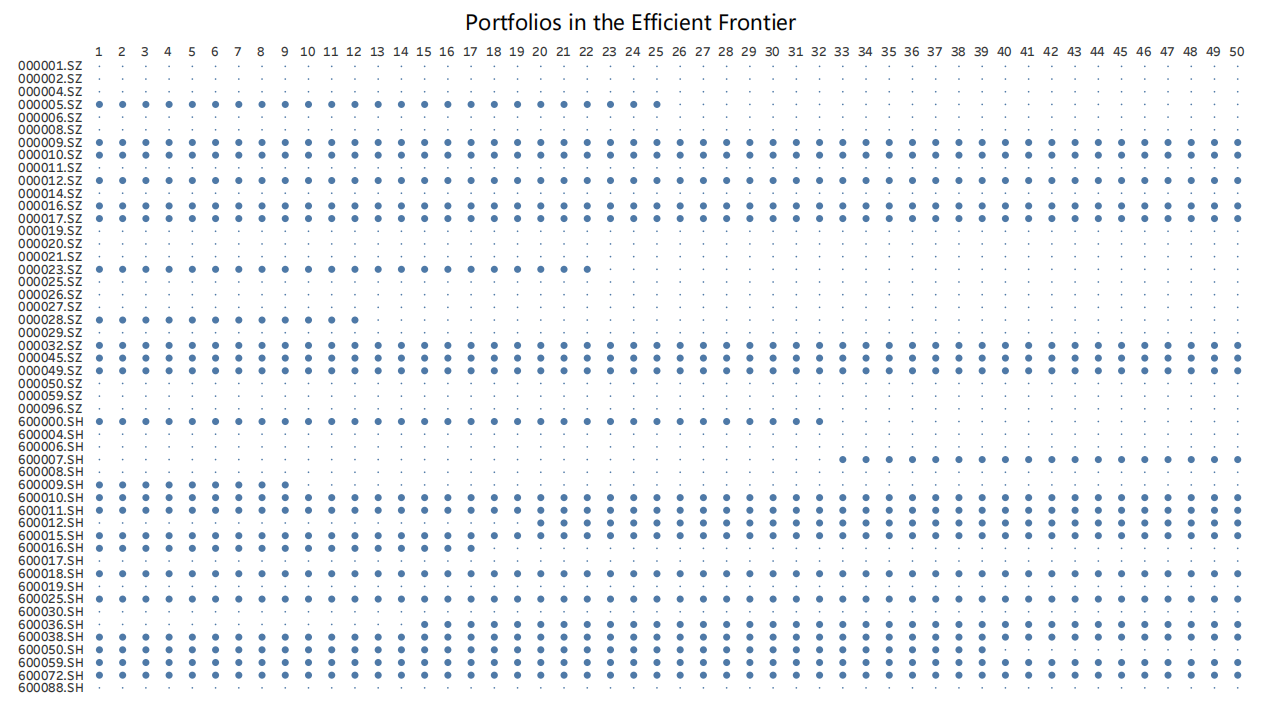
\includegraphics[width = 0.9\textwidth]{figures/Fig 3.png}
	\caption{The 50 portfolios form the efficient frontier for the sample stocks from 9 January 2020 to 13 December 2021. Each column is the optimal portfolio for a given return. If the stock is included in the portfolio it is shown as a blue dot, otherwise it is blank.}
	\label{fg3}
\end{figure*} 

\section{Predictive Machine Learning Model}\label{sec5}
\subsection{Training and Test Set}\label{sec5sub1}
\hspace{1.5em} In order to get more training and test data, we split up the target time period, from 9 January 2020 to 28 February 2024, into three time periods by time series and obtain the effective frontier of each time period to calculate the labels of the target stocks in these three time periods.

We split up the matrix of daily returns $X$ by rows to get a training and test set \cite{buhler2023efficient}. The first $t$ rows of $X$ are denoted as $X_{train}$, and the remaining $T-t$ rows are denoted as $X_{test}$. As a result, a dataset containing the daily returns of the fifty stocks and their corresponding labels can be used for machine learning. We finally split the data to three time period and get three matrix with $50 \times 267$ size. We choose two of the $50 \times 267$ matrix as the training set for machine learning, and one $50 \times 267$ matrix as the test set for machine learning.

For the label y of the stock, we need to convert the text-based classification labels into numeric form. We define the labels of the stocks according to the following equation:
\begin{align}
	Y_{train/test}=\begin{cases}
		& \text 0 \hspace{1em}if \hspace{0.5em}label='Loser' \\
		& \text 1 \hspace{1em}if \hspace{0.5em}label='None'\\
		& \text 2 \hspace{1em}if \hspace{0.5em}label='Winner'
	\end{cases}
\label{eq8}
\end{align}

In addition, in order to improve the accuracy and efficiency of machine learning, we process the data in the training and test sets. When the possible range value of a feature is larger, its weight may be smaller, which leads to an uneven distribution of the feature scatterplot. The contour plot of the cost function may exhibit an extreme elongation, making it difficult for the gradient descent to find the target. Therefore, we use feature scaling to normalize the feature X \cite{fu2018machine}. With this processing, we can control the feature, the daily return of the stock, between -1 and 1 used to make the gradient drop faster. We choose the following normalization method:
\begin{align}
	X_{i,t}' =\frac{X_{i,t}-\mu_{t}}{\sigma _{t}} 
\label{eq9}
\end{align}

\subsection{Long Short-term Memory Neural Network}\label{sec5sub2}
\hspace{1.5em}The architecture we chose for the neural network is the Long Short-Term Memory (\textit{LSTM}) network \cite{1997Long}, which is a type of Recurrent Neural Network (\textit{RNN}), since the literature \cite{2018Deep,2020Portfolio} demonstrated to us that LSTM network architectures have high predictive power for financial data, especially in equity securities. Predicting the labels of stocks under each optimal portfolio on the efficient frontier should require a more complex network architecture than predicting stock prices or returns based on time series alone, but the underlying logic should be similar.

Python programming language has been used to design portfolio and LSTM models. We mainly use Tensorflow and Keras frameworks to design neural networks and back-portion \cite{Aur2017Hands}. The basic architecture of LSTM network enables the neural network to maintain the original information in some specially designed storage units, namely gates. The gate is a binary variable (0, 1) with 0 representing the closed state and no information allowed to pass and 1 representing the open state and allowing all information to pass. Gate is actually a layer of full connectivity in the LSTM network, the input is a vector, and the output is a real vector between 0 and 1. Indicates that information is allowed to pass in a certain proportion.

LSTM implements three gate computations, forgetting gate, input gate, and output gate, which are used to protect and control unit states. The forgetting gate decides how much historical information is retained and uses sigmoid as the activation function output 0 and 1 to decide to retain or discard. The input door determines how much input from the current moment remains to the cell state from the current moment. It uses the sigmoid layer to decide what value to update, and then uses the tanh layer to update the information. The output gate determines how many outputs are available at the current moment, determines which parts of the output through the sigmoid layer, and then multiplies the output determined information with the results of the tanh function. Figure \ref{fg4} visualizes how LSTM works inside a cell.
\begin{figure*}[h]
	\centering    
	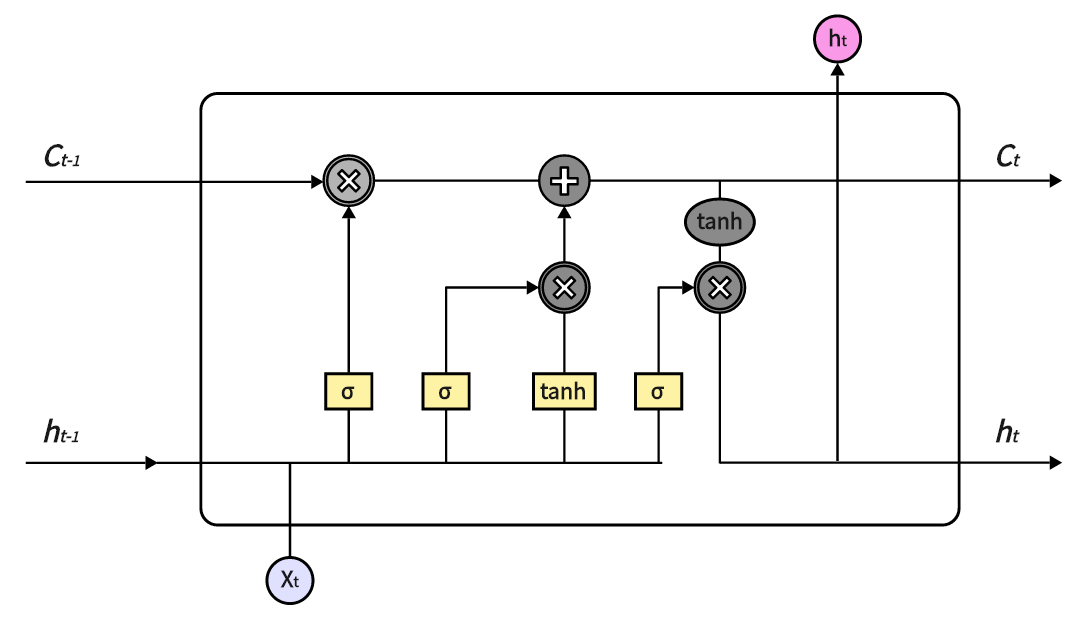
\includegraphics[width = 0.8\textwidth]{figures/Fig 4.png}
	\caption{The internal structure of the LSTM neural network, shows the detailed processing of information through the input gate, the forget gate and the output gate.}
	\label{fg4}
\end{figure*} 

We use the back-propagation algorithm to train the parameters of LSTM. We make little adjustments to the architecture of the LSTM neural network and use a regularization parameter of 0.001 for each layer of the neural network for L2-type regularization to avoid over-fitting \cite{2009L2}. Our network has four layers:
\begin{enumerate}
	\item \textbf{Input Layer:} The single dimension input layer is given $X_{\text{train}}$.We first use a dense layer as the input layer to receive the training set. The layer has forty nodes, and the activation function is ReLU, which receives the daily return of stocks over the past 259 days and finds some features.
	\item \textbf{LSTM Layer:} We selected 25 hidden nodes in this layer. The state activation function is the hyperbolic tangent function. The gate activation function is the sigmoid function. This layer is used to selectively output data from the previous layer to avoid long-term dependence problems.
	\item \textbf{Fully Connected Layer:} This layer is a dense layer with 15 nodes and the activation function is ReLU. This layer accepts the output of the LSTM layer and reshapes the data in preparation for the classification of the next layer.
	\item \textbf{Output Layer:} This layer has three nodes for classifying all data from the upper layer to prepare for outputting three types of labels for stocks. The activation function of this layer is Softmax, it outputs the probability of labels 0, 1, and 2 which is used to determine whether the type of stock is a winner, loser, or none.
\end{enumerate}

Based on the training set, X-train as the data and Y-train as the label, we train the parameters of the network. Then, we input X-test, and obtain the output of it as Y-predict with trained network and compare it with Y-test to determine the performance of the network. Figure \ref{fg5} demonstrates the network architecture while Table \eqref{tab3} demonstrate the network hyperparameters \cite{smith2018dont}.
\begin{table}[htbp]
	\renewcommand{\arraystretch}{1.25}
	\centering
	\begin{tabular}{@{}ll@{}}
		\toprule
		\textbf{Hyperparameter} & \textbf{Value} \\ 
		\midrule
		Initial Learning Rate  &  0.0005 \\
		% \midrule
		Decay Factor &  2.5e-06\\
		% \midrule
		Epsilon     & 1.0000e-08\\
		% \midrule
		Beta 1 &  0.9000 \\ 
		% \midrule
		Beta 2 & 0.9990 \\
		% \midrule
		L2 Regularization & 0.001\\
		% \midrule
		Epochs & 200 \\
		% \midrule
		Batch Size &  50\\
		\botrule
	\end{tabular}
	\caption{Hyperparameters for neural network. }
	\label{tab3}
\end{table}

\begin{figure*}[h]
	\centering    
	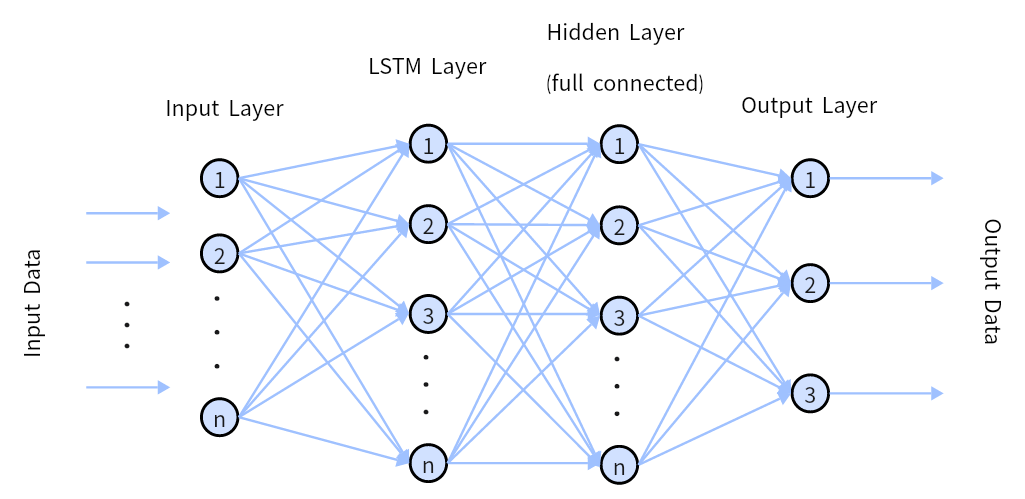
\includegraphics[width = 0.8\textwidth]{figures/Fig 5.png}
	\caption{\centering{The schematic diagram of our LSTM model.}}
	\label{fg5}
\end{figure*} 

\section{Result and Application}\label{sec6}
In this section, the detailed results of the neural network model are presented and analyzed in terms of statistical and practical aspects.
\subsection{Model Analysis}\label{sec6sub1}
\hspace{1.5em}We first use the keras framework in python on the trained model to see the state of each layer of the neural network during the training process. We get the shape of the output matrix of each layer of the neural network and the number of parameters that need to be trained for each layer as shown in Table \eqref{tab4}.

\begin{table}[htbp]
	\renewcommand{\arraystretch}{1.25}
	\centering
	\begin{tabular}{@{}L{1cm}rr@{}}
			\toprule
			\textbf{Layer (Type)}  & \textbf{Output Shape}  & \textbf{Param \#}  \\ 
			\botrule
			dense (Dense)& (50,267,40) & 80  \\ 
			\midrule
			lstm (LSTM)     & (50,25)&   6600 \\ 
			\midrule
			dense\_1 (Dense)& (50,15) & 390 \\ 
			\midrule
			dense\_2 (Dense)   &  (50,3)  &  48 \\ 
			\midrule
			\multicolumn{3}{l}{Total parameters: 7118 (27.80 KB)} \\
			\multicolumn{3}{l}{Trainable parameters: 7118 (27.80 KB)} \\
			\multicolumn{3}{l}{Non-trainable parameters: 0 (0 Byte)} \\
			\botrule
	\end{tabular}
	\caption{Basic training information of neural network. }
	\label{tab4}
\end{table}

In machine learning iterations, we use the Sparse Categorical Crossentropy Function \cite{2005A} as the loss function because the model is essentially a multiclassification problem based on the softmax algorithm and the label is an integer instead of one-hot code. This loss function describes the gap between two distributions, with the smaller the cross-entropy the closer the hypothesised distribution is to the true distribution. We plot the trend of the value of the loss function with the number of training sessions, as shown in Fig \ref{fg6}. The loss function starts to show a convergence trend after 50 iterations and keeps converging until 200 iterations. This indicates that the Adan optimizer \cite{2014Adam} is constantly approaching the local minimum according to a variable learning rate, and there is no gradient vanishing or gradient explosion.
\begin{figure}[htbp]
	\centering    
	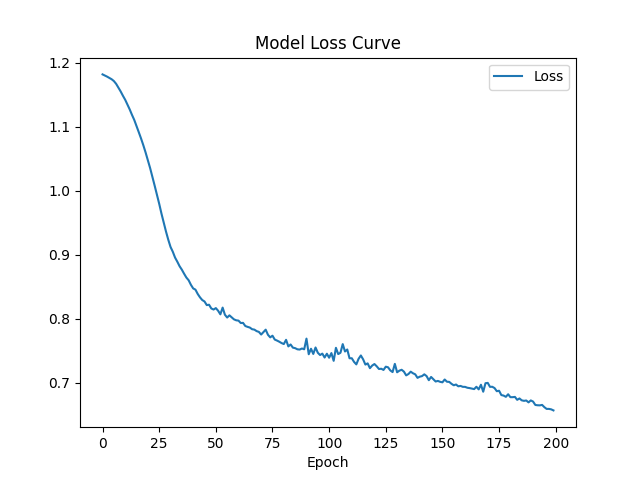
\includegraphics[width = 0.5\textwidth]{figures/Fig 6.png}
	\caption{\centering{The loss curve of our model versus epochs.}}
	\label{fg6}
\end{figure} 
\subsection{Statistic Analysis}\label{sec6sub2}
\hspace{1.5em}We input the data from the training and test sets into the trained model to get the model's predictions about $X_{train}$ and $X_{test}$. Since the model predictions are in the form of probabilities of each stock being each of the three labels, in Python we process them using argmax in the numpy framework to get direct predictions of the target stock labels. We construct a multiclassification confusion matrix to visualize the precision and recall of the machine learning test set as shown in Fig \ref{fg7}.

Based on this result, we can see that the overall accuracy of the model is 62\% on the test set. It is worth mentioning that the model's prediction on the training set yields an accuracy of 79\%. The precision and recall on the test set are calculated as follows: 
\begin{align}
	Precision=\frac{1}{3}  {\textstyle \sum_{i=0}^{2}}\frac{TP_{i}}{TP_{i}+FP_{i}}  \\
	Recall=\frac{1}{3}  {\textstyle \sum_{i=0}^{2}}\frac{TP_{i}}{TP_{i}+FN_{i}}  
\end{align}
The result of the calculation is: Precision = $\frac{1}{3}$ $\times$ (0.935 + 0 + 0.143) = 0.3673 and Recall = $\frac{1}{3}$ $\times$ (0.644 + 0 + 0.4) = 0.3481.
Based on this result and Fig \ref{fg7}, we can see that the model performs moderately well in terms of overall accuracy and is quite accurate in predicting stocks with a label of 0. However, the model is less accurate for stocks labeled 1 and 2. It means that when a stock is a loser, it's highly possible that the model will report it correctly. Nevertheless, if a stock is a winner, the model maybe mistake it as a loser with a moderate probability and when a stock is neither a loser nor a winner, it's highly difficult for the model to correctly report it.  
\begin{figure}[htbp]
	\centering    
	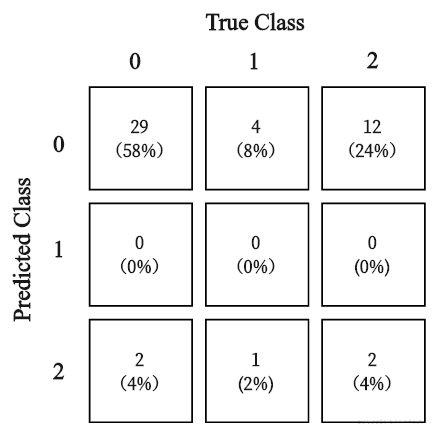
\includegraphics[width = 0.3\textwidth]{figures/Fig 7.png}
	\caption{The confusion matrix predicted by the model on the test set is shown. The categories are 0, 1 and 2, where 0 means loser, 1 means none, and 2 means winner.}
	\label{fg7}
\end{figure} 
\subsection{Model Application}\label{sec6sub3}
\hspace{1.5em}To test the practical used ability of our trained neural network model, we establish a test.

First, we selected fifteen stocks from the Tushare database that have been consistently high in recent days as targets and applied a call to their daily pre-adjusted closing price from 15 February 2023 to 28 March 2024 to calculate their daily returns.
\begin{figure*}[htbp]
	\centering    
	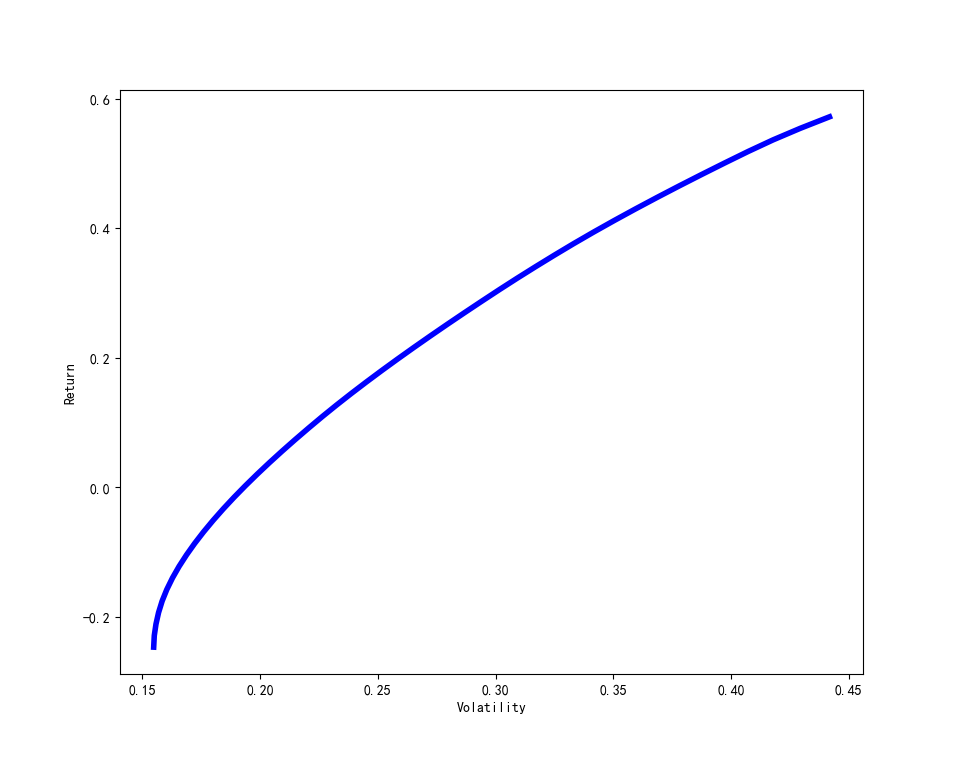
\includegraphics[width = 0.8\textwidth]{figures/Fig 8.png}
	\caption{Efficient frontier of all the 15 stocks using daily returns from 15 February 2023 to 28 March 2024 (Returns and Volatility are processed as annualized by 252 trading day).}
	\label{fg8}
\end{figure*} 

We asked a subject with previous experience in stock investment to choose his favourable portion of stocks from these 15 stocks to invest in any of his own ways. At the same time, we use the trained model to predict the losers and winners among these 15 stocks based on their daily returns over the target time period while we invest only in the winners. Table \eqref{tab5} shows the ticker symbols of these 15 stocks, the manually selected stocks and the labels predicted by the model.
\begin{table}[htbp]
	\centering  
	\begin{tabular}{|c|c|c|}  
		\hline  % 表格的横线
		& & \\[-6pt]  %可以避免文字偏上来调整文字与上边界的距离
		\textbf{Stock Code}&\textbf{Artificial selection}&\textbf{Pre-Label} \\  
		\hline
		& & \\[-6pt]
		\textbf{000049.SZ}&N&Loser \\
		\hline
		& & \\[-6pt]
		\textbf{600733.SH}&Y&Winner \\
		\hline
		& & \\[-6pt]
		\textbf{000969.SZ}&N&Loser \\
		\hline
		& & \\[-6pt]
		\textbf{000099.SZ}&N&Winner \\
		\hline
		& & \\[-6pt]
		\textbf{600211.SH}&N&Loser \\
		\hline
		& & \\[-6pt]
		\textbf{600165.SH}&N&Winner \\
		\hline
		& & \\[-6pt]
		\textbf{600233.SH}&N&Winner \\
		\hline
		& & \\[-6pt]
		\textbf{000012.SZ}&Y&Loser \\
		\hline
		& & \\[-6pt]
		\textbf{002171.SZ}&Y&Loser \\
		\hline
		& & \\[-6pt]
		\textbf{600917.SH}&N&Loser\\
		\hline
		& & \\[-6pt]
		\textbf{002049.SZ}&N&Loser \\
		\hline
		& & \\[-6pt]
		\textbf{002747.SZ}&N&Loser \\
		\hline
		& & \\[-6pt]
		\textbf{002985.SZ}&N&Loser \\
		\hline
		& & \\[-6pt]
		\textbf{002929.SZ}&Y&Loser \\
		\hline
		& & \\[-6pt]
		\textbf{002414.SZ}&Y&Loser \\
		\hline
	\end{tabular}
	\caption{The code, artificial selection and predicted label of the 15 stocks} 
	\label{tab5}
\end{table}

Based on the five stocks selected by the subjects and the four winner stocks predicted by the model, we construct the efficient frontier for each of these two investment samples, as shown in Fig \ref{fg9}. Rational investors will make different portfolios on the efficient frontier according to their risk aversion.
\begin{figure*}[htbp]
	\centering    
	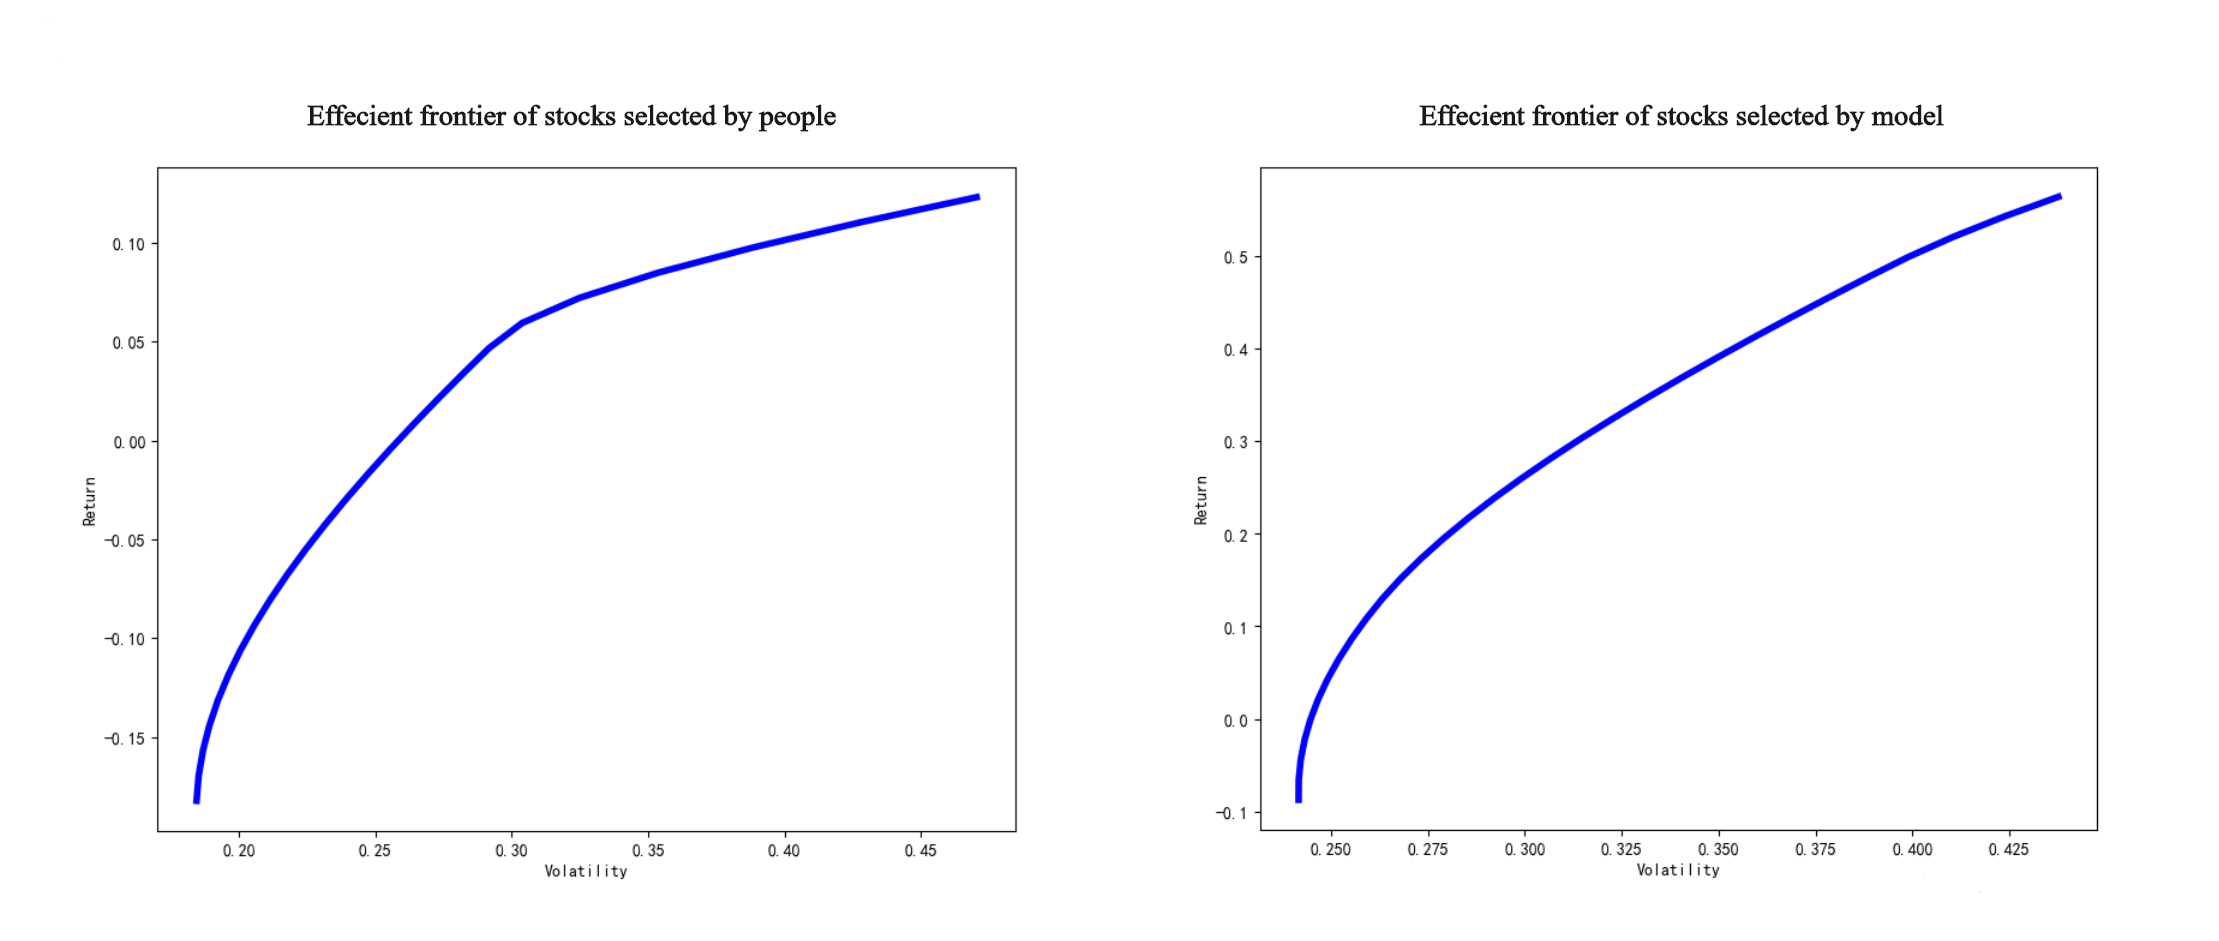
\includegraphics[width = 0.8\textwidth]{figures/Fig 9.png}
	\caption{Efficient frontiers of stocks selected by people and model using daily returns from 15 February 2023 to 28 March 2024 (Returns and Volatility are processed as annualized by 252 trading day)}
	\label{fg9}
\end{figure*} 

We can visualize that the portfolio returns are roughly distributed between -0.2 and 0.1 on the efficient frontier consisting of the five stocks chosen by the subjects, and the corresponding variance is roughly between 0.2 and 0.45. On the efficient frontier consisting of the four winning stocks chosen by the model, the portfolio returns are roughly distributed between -0.1 and 0.6, corresponding to a variance of roughly 0.25 to 0.45. This result implies that at nearly the same level of variance, the returns of the portfolio consisting of the four winner stocks selected by the neural network model are much better than those of the portfolio consisting of the five stocks selected by the subjects. At the same time, the effective frontier of the stocks selected by the model is almost the same as the effective frontier of all these 15 stocks except for a slight increase in variance. However, the increase of variance is an inevitable consequence of reducing the number of stocks as investment targets.

This finding shows the good results of our model in practical application. It can help us to quickly target winner stocks to invest in the whole stock market, and its return is far better than the stocks chosen by human beings according to their own preference. Meanwhile, in the real world, the stock market is very large and may contain thousands of or even more stocks, and it is difficult for us to construct an efficient frontier with all the stocks as investment objects. This is because a huge number of stocks will generate a covariance matrix that is large and dense, reducing the efficiency of the algorithm's operation. Our model avoids this problem by simply inputting the daily returns for a recent period of time, and we can quickly determine if the stock has the potential to be included in our portfolio. Furthermore, when a new stock flows into the stock market, we can use its daily returns in the short term to determine whether the stock is more likely to be a winner, a loser, or none.

\section{Discussion}\label{sec7}
\hspace{1.5em}In this study, we analyzed fifty randomly selected stocks using the Markowitz mean-variance model. Based on their performance in portfolios on the efficient frontier, we categorize them to obtain the relevant dataset. We construct a well-designed LSTM neural network to perform supervised machine learning on the labeled dataset. The model has an accuracy of 79\% on the training set and 62\% on the test set. The trained model could more efficiently determine whether a stock is worth investing in a real stock market containing a huge number of stocks. By investing in the stocks selected by the model, the investor can achieve a significantly higher return for a specific level of risk. Furthermore, for new stocks coming into the stock market, we can determine whether the stock can be included in our portfolio in a relatively short period of time.

However, we find that the model's predictions for stocks with label 1 and 2, particular label 1 that are neither losers nor winners, are very ambiguous. In other words, the model is more likely to predict 0 for stocks that are actually with label 1 and 2. This phenomenon may be due to the fact that the dataset we used for training is a skewed dataset. The stocks are mostly losers and a small percentage of them are winners, while stocks that are neither losers nor winners account for only a highly small percentage.

Most of the current researchers in this area use artificial neural networks, such as LSTM, to make a stock price or return prediction on a time series. Moreover, some of researchers have also made complex definitions for the attributes of the stock itself and moved to making predictions on the attributes of the stock as the defined labels. Perhaps adding more features to the stock, first using a genetic algorithm for feature screening and then using a larger dataset for deep neural network training would result in a model that is more accurate and more widely used.
\section{Conclusion}\label{sec8}
\hspace{1.5em}We randomly select 50 stocks in the domestic Shanghai and Shenzhen stock markets as the study object. The Tushare database provides the pre-adjusted closing prices of the target stocks. Through Markowitz capital portfolio, we study the mean-variance model on the target stocks to get the portfolio on the efficient frontier. Based on the number of stocks being invested (with weights above a threshold) in the portfolio on the efficient frontier, we classify the stocks as Winners, Losers, and None to get the training and test sets for machine learning. The dataset consists of the daily return of a stock over a specific time period and its corresponding label.

We build a neural network with four layers, accept the dataset with a dense layer, study the daily returns of stocks in a time series with an LSTM, prepare for classification with a fully connected layer, and use the Softmax function for output. We set suitable hyperparameters and train this multilayer neural network model with the obtained dataset by supervised learning.

Main conclusions can be drawn from this work as follows. Machine learning can be used to predict whether stocks in a portfolio are losers or winners. Our neural network model has a relatively high accuracy on the dataset and demonstrate significantly higher efficiency and expected returns than manually selecting stocks for portfolios in real practice. Furthermore, most people in the market today use Markowitz portfolio theory directly to study stock selection. However, the large and dense covariance matrix generated by a large number of stocks in the real stock market makes portfolio selection from the whole market almost impossible. Machine learning based on mean-variance model can solve this challenge by efficiently selecting "better" stocks to invest.
\clearpage
\onecolumn
\backmatter
\section*{Declarations}\label{sec9}

% . Other declarations include Ethics approval, Consent, Data, Material and/or Code availability and Authors’ contribution statements.
\subsection*{1 Funding}\label{sec9sub1}
The author declare that no any funds are received during the Final Year Project research.

\subsection*{2 Data}\label{sec9sub2}
All the financial data, such as the stock code, the pre-adjusted daily closing price, sort of things, was collected from the website Tushare. We use Tushare library through python to directly call the needed data from Tushare by API . The website is \url{https://tushare.pro/}.

\noindent
%%===================================================%%
%% For presentation purpose, we have included        %%
%% \bigskip command. please ignore this.             %%
%%===================================================%%
\bigskip


\begin{appendices}
\section{Notations}\label{secA1}
Here we list the symbols and notations used in our paper, as shown in Table \ref{taba1}.
\begin{table*}[htbp]
	\begin{tabular}{cl}
			\toprule
			\multicolumn{1}{m{3cm}}{\centering Symbol}
			&\multicolumn{1}{m{8cm}}{Definition}\\
			\midrule
			$r_{i,t}$&returns of stock $i$ on day $t$\\
			$p_{i,t}$&price of stock $i$ on day $t$\\
			$\mu_{i}$&mean returns of stock $i$, forming matrix $\mu$\\
			$w_{i}$&weight of stock $i$ in a portfolio, forming matrix $w$ \\
			$\mathbb{E}(R)$ &expected whole returns on the portfolio\\
			$\sigma _{i}$ &the standard deviation of stock $i$\\
			$\sigma _{i,j}$ &covariance between stock $i$ and $j$, forming covariance matrix cov(R)\\
			$\mathbb{V}(R)$ &variance of a portfolio\\
			$\bar{R}$ &target returns\\
			$I$ &length of time series data\\
			$N$ &number of sample stocks\\
			$x_{i,t}$ &returns of stock $i$ on day $t$\\
			$\mu_{t}$ &mean returns of stocks on day $t$\\
			$\sigma_{t}$ &standard deviation of stock returns on day $t$\\
			$TP_{i} $ &number of true positive for $i$ type label\\
			$FP_{i} $ &number of false positive for $i$ type label\\
			$FN_{i} $ &number of false negative for $i$ type label\\
	\end{tabular}
	\label{taba1}
\end{table*}
\clearpage

\section{Activation and Loss Functions}\label{secA2}
The activation and loss functions we use to build LSTM neural network are shown in Table \ref{taba2}. $m$ is the sample size, $y_{i}$ is the actual value of class $i$ while $f(x_{i})$ is the predicted value of class $i$. The letter $z$ in the formula table is defined by the following equation: $z=\overrightarrow{w}\overrightarrow{x} +b$
\begin{table}[htbp]
	\renewcommand{\arraystretch}{2}
	\centering
	\resizebox{.5\textwidth}{!}{
		\begin{tabular}{@{}L{2.1cm}l@{}}
			\toprule
			Function & Equation \\ 
			\midrule
			Sigmoid & $f_{\overrightarrow{w},b } (\overrightarrow{x} )=\dfrac{1}{1+e^{-z} } $ \\[2.5em]
			% \midrule
			Softmax & $f_{\overrightarrow{w},b } (\overrightarrow{x_{i}} )=\dfrac{e^{z_{i}}}{\sum_{j-1}^{J} e^{-z_{j}} } $\\[2.5em]
			% \midrule
			Hyperbolic Tangent      & $f(x)=\dfrac{e^x-e^{-x}}{e^x+e^{-x}}$ \\[2em]
			% \midrule
			ReLU & $f(x)=max(0,x)$\\[2em]
			% \midrule
			Sparse Cross Entropy Loss & $Q=-\dfrac{1}{m} \sum_{i=1}^{m}(y_{i}ln(f(x_{i}) )+(1-y_{i})ln(1-f(x_{i}))$\\
			\botrule
	\end{tabular}}
	\caption{Activation and loss functions for training networks. $\eta$ is the number of samples, $K$ is total number of classes, $\beta_i$ is the weight for class $i$, $y_i$ is the actual value for class $i$, and $\hat{y}_i$ is the prediction value for class $i$.}
	\label{taba2}
\end{table}
\clearpage

\section{Code}\label{secA3}
\subsection{Code block 1}\label{SecA3sub1}
The code of the program in the mean-variance model and efficient frontier part is shown below:
\begin{lstlisting}[language=Python,numbers=left, 
	numberstyle= \tiny, 
	keywordstyle= \color{ blue!70},
	commentstyle= \color{red!50!green!50!blue!50}, 
	frame=shadowbox, % 阴影效果
	rulesepcolor= \color{ red!20!green!20!blue!20} ,
	escapeinside=``, % 英文分号中可写入中文
	xleftmargin=2em,xrightmargin=2em, aboveskip=1em,
	framexleftmargin=2em]
	import numpy as np
	import pandas as pd
	import tushare as ts
	import matplotlib.pyplot as plt
	
	pd.set_option('display.max_rows',10000)
	pd.set_option('display.max_columns',10000)
	np.set_printoptions(threshold=np.inf)
	plt.rcParams['font.sans-serif'] = ['SimHei'] 
	plt.rcParams['axes.unicode_minus'] = False 
	
	My_token = '3b903a2c73297d69aaf9caf8adc356249b787a56182cdba4e65a48a6'
	pro = ts.pro_api(My_token)
	
	stock_code_list = ['000001.SZ', '000002.SZ', '000004.SZ', '000005.SZ', '000006.SZ', '000008.SZ', '000009.SZ', '000010.SZ', '000011.SZ', '000012.SZ', '000014.SZ', '000016.SZ', '000017.SZ', '000019.SZ', '000020.SZ', '000021.SZ', '000023.SZ', '000025.SZ', '000026.SZ', '000027.SZ', '000028.SZ', '000029.SZ', '000032.SZ', '000045.SZ', '000049.SZ', '000050.SZ', '000059.SZ', '000096.SZ', '600000.SH', '600004.SH', '600006.SH', '600007.SH', '600008.SH', '600009.SH', '600010.SH', '600011.SH', '600012.SH', '600015.SH', '600016.SH', '600017.SH', '600018.SH', '600019.SH', '600025.SH', '600030.SH', '600036.SH', '600038.SH', '600050.SH', '600059.SH', '600072.SH', '600088.SH']
	prices = pd.DataFrame() 
	for stock_code in stock_code_list:
	if 'trade_date' not in prices.columns:
	prices['trade_date'] = ts.pro_bar(ts_code=stock_code, api=pro, adj='qfq', start_date='20200109',end_date='20240228')['trade_date']
	prices[stock_code] = ts.pro_bar(ts_code=stock_code, api=pro, adj='qfq', start_date='20200109',end_date='20240228')['close']
	
	prices.dropna(inplace=True) 
	prices.set_index('trade_date', inplace=True)
	prices.sort_index(ascending=True, inplace=True)
	
	asset_nums = prices.shape[1]
	returns = np.log(prices/prices.shift(1))
	
	def port_rets(weights):
	return np.sum(returns.mean() * weights) * 252  
	
	def port_vols(weights):
	return np.sqrt(np.dot(weights.T, np.dot(returns.cov() * 252, weights))) 
	
	import scipy.optimize as sco
	def min_func_sharpe(weights):
	return -port_rets(weights)/port_vols(weights)
	cons = {'type': 'eq', 'fun': lambda x: np.sum(x) - 1} 
	bnds = tuple((0, 1) for x in range(asset_nums))
	weights0 = np.array(asset_nums * [1./asset_nums, ]) 
	opts = sco.minimize(min_func_sharpe, weights0, bounds=bnds, constraints=cons, method='SLSQP')

	optv = sco.minimize(port_vols, weights0, bounds=bnds, constraints=cons, method='SLSQP')
	
	cons = ({'type': 'eq', 'fun': lambda x: port_rets(x) - tret}, {'type': 'eq', 'fun': lambda x: np.sum(x) - 1})  
	bnds = tuple((0, 1) for x in range(asset_nums)) 
	weights00 = np.array(asset_nums * [1./asset_nums, ]) 
	trets = np.linspace(0, 0.45, 50)
	tvols = []
	weights = []
	for tret in trets:
	res = sco.minimize(port_vols, weights00, method='SLSQP', bounds=bnds, constraints=cons)
	tvols.append(res['fun'])
	weights.append(res['x'])
	tvols = np.array(tvols)
	ind = np.argmin(tvols)
	evols = tvols[ind:]
	erets = trets[ind:]
	
	returns.cov().to_excel('Covariance Table.xlsx',index=True)
	np.vstack(returns.std(),returns.mean()).to_excel('Standard Deviation Table.xlsx',index=True)
	prices.to_excel('Daily Closing Price Table.xlsx',index=True)
	weights = np.array(weights)
	weights1 = pd.DataFrame(weights)
	weights1.to_excel('All Weights.xlsx', index=True)
	returns.to_excel('Return.xlsx',index=True)
	
	plt.figure(figsize=(10, 8))
	plt.plot(evols, erets, 'b', lw=4.0)
	plt.plot(port_vols(opts['x']), port_rets(opts['x']), 'y*', markersize=12.0)
	plt.xlabel('Volatility')
	plt.ylabel('Return')
	plt.show()
\end{lstlisting}
\clearpage
\subsection{Code block 2}\label{secA3sub2}
The code of the program in the neural network machine learning part is shown below:
\begin{lstlisting}[language=Python,numbers=left, 
	numberstyle= \tiny, 
	keywordstyle= \color{ blue!70},
	commentstyle= \color{red!50!green!50!blue!50}, 
	frame=shadowbox, % 阴影效果
	rulesepcolor= \color{ red!20!green!20!blue!20} ,
	escapeinside=``, % 英文分号中可写入中文
	xleftmargin=2em,xrightmargin=2em, aboveskip=1em,
	framexleftmargin=2em]
	import pandas as pd
	import numpy as np
	import tensorflow as tf
	import matplotlib.pyplot as plt
	
	df1 = pd.read_excel('machine learning data 0.xlsx')
	df2 = pd.read_excel('machine learning data 3.xlsx')
	df3 = pd.read_excel('Example Returns 1.xlsx')
	
	x_train = df1.values[0:100,1:268]
	for i in range(x_train.shape[1]):
	mean1 = np.mean(x_train[:,[i]])
	std1 = np.std(x_train[:,[i]])
	x_train[:,[i]] = (x_train[:,[i]]-mean1)/std1
	y_train = df1.values[0:100,268]
	
	x_test = df2.values[0:50,1:268]
	for j in range(x_test.shape[1]):
	mean2 = np.mean(x_test[:,[j]])
	std2 = np.std(x_test[:,[j]])
	x_test[:,[j]] = (x_test[:,[j]]-mean2)/std2
	y_test = df2.values[0:50,268]
	
	x_example = df3.values[0:15,1:268]
	for k in range(x_test.shape[1]):
	mean3 = np.mean(x_example[:,[k]])
	std3 = np.std(x_example[:,[k]])
	x_example[:,[k]] = (x_example[:,[k]]-mean3)/std3
	
	x_test = x_test.astype('float32')
	x_train = x_train.astype('float32')
	x_example = x_example.astype('float32')
	y_test = y_test.astype('int')
	y_train = y_train.astype('int')
	x_train,x_test,x_example = tf.reshape(x_train,[len(x_train),267,-1]),tf.reshape(x_test,[len(x_test),267,-1]),tf.reshape(x_example,[len(x_example),267,-1])
	
	model = tf.keras.models.Sequential([
	tf.keras.layers.Dense(units=40,activation=tf.nn.relu,kernel_regularizer=tf.keras.regularizers.l2(0.001)),
	tf.keras.layers.LSTM(units=25,kernel_regularizer=tf.keras.regularizers.l2(0.001)),
	tf.keras.layers.Dense(units=15, activation=tf.nn.relu,kernel_regularizer=tf.keras.regularizers.l2(0.001)),
	tf.keras.layers.Dense(units=3, activation=tf.nn.relu,kernel_regularizer=tf.keras.regularizers.l2(0.001))
	], name="LSTM")
	
	loss_function = tf.keras.losses.SparseCategoricalCrossentropy(from_logits=True)

	model.compile(optimizer=tf.keras.optimizers.Adam(learning_rate=0.0005), loss=loss_function, metrics=['accuracy'])

	history = model.fit(x_train, y_train,
	epochs=200,
	batch_size=50,
	validation_data=(x_test, y_test))
	model.summary()
	model.save('Stock Prediction Model.keras')
	logits1 = model(x_test)
	logits2 = model(x_train)
	logits3 = model(x_example)
	y_test_predict_prob = tf.nn.softmax(logits1)
	y_train_predict_prob = tf.nn.softmax(logits2)
	y_example_predict_prob = tf.nn.softmax(logits3)
	y_test_predict = np.argmax(y_test_predict_prob,axis=1)
	y_train_predict = np.argmax(y_train_predict_prob,axis=1)
	y_example_predict = np.argmax(y_example_predict_prob,axis=1)
	count1 = sum(1 for x, y in zip(y_test_predict,y_test) if x == y)
	count2 = sum(1 for x, y in zip(y_train_predict,y_train) if x == y)
	print('Accuracy for test set:',count1/50)
	print('Accuracy for train set:',count2/100)
	
	y_train_predict = pd.DataFrame(y_train_predict)
	y_test_predict = pd.DataFrame(y_test_predict)
	y_example_predict = pd.DataFrame(y_example_predict)
	y_train_predict.to_excel('Result train.xlsx', index=True)
	y_test_predict.to_excel('Result test.xlsx', index=True)
	y_example_predict.to_excel('Result example.xlsx', index=True)
	
	def print_history(history):
	plt.plot(history.history['loss'])
	plt.title('Model Loss Curve')
	plt.xlabel('Epoch')
	plt.legend(['Loss'])
	plt.show()
	
	print_history(history)
	tf.keras.utils.plot_model(model, "my_first_model_with_shape_info.png", show_shapes=True)
\end{lstlisting}
\end{appendices}
\clearpage
\twocolumn
%%===========================================================================================%%
%% If you are submitting to one of the Nature Portfolio journals, using the eJP submission   %%
%% system, please include the references within the manuscript file itself. You may do this  %%
%% by copying the reference list from your .bbl file, paste it into the main manuscript .tex %%
%% file, and delete the associated \verb+\bibliography+ commands.                            %%
%%===========================================================================================%%

% \newpage
\bibliographystyle{sn-aps}
\bibliography{ref}% common bib file
%% if required, the content of .bbl file can be included here once bbl is generated
%%\input sn-article.bbl


\end{document}
